
%% CodeInk, UIST 2014 Paper Submission
%% 2014/04/01


\documentclass{sigchi}

% Use this command to override the default ACM copyright statement (e.g. for preprints). 
% Consult the conference website for the camera-ready copyright statement.


%% EXAMPLE BEGIN -- HOW TO OVERRIDE THE DEFAULT COPYRIGHT STRIP -- (July 22, 2013 - Paul Baumann)
% \toappear{Permission to make digital or hard copies of all or part of this work for personal or classroom use is 	granted without fee provided that copies are not made or distributed for profit or commercial advantage and that copies bear this notice and the full citation on the first page. Copyrights for components of this work owned by others than ACM must be honored. Abstracting with credit is permitted. To copy otherwise, or republish, to post on servers or to redistribute to lists, requires prior specific permission and/or a fee. Request permissions from permissions@acm.org. \\
% {\emph{CHI'14}}, April 26--May 1, 2014, Toronto, Canada. \\
% Copyright \copyright~2014 ACM ISBN/14/04...\$15.00. \\
% DOI string from ACM form confirmation}
%% EXAMPLE END -- HOW TO OVERRIDE THE DEFAULT COPYRIGHT STRIP -- (July 22, 2013 - Paul Baumann)

\toappear{In submission to UIST 2014}

% Arabic page numbers for submission. 
% Remove this line to eliminate page numbers for the camera ready copy
\pagenumbering{arabic}

\usepackage{comment}

% Load basic packages
\usepackage{balance}  % to better equalize the last page
\usepackage{graphics} % for EPS, load graphicx instead
\graphicspath{{img/}}
% and their extensions so you won't have to specify these with
% every instance of \includegraphics
\DeclareGraphicsExtensions{.pdf,.jpeg,.png}
\usepackage{times}    % comment if you want LaTeX's default font
\usepackage{url}      % llt: nicely formatted URLs

% llt: Define a global style for URLs, rather that the default one
\makeatletter
\def\url@leostyle{%
  \@ifundefined{selectfont}{\def\UrlFont{\sf}}{\def\UrlFont{\small\bf\ttfamily}}}
\makeatother
\urlstyle{leo}

\usepackage{array}


% To make various LaTeX processors do the right thing with page size.
\def\pprw{8.5in}
\def\pprh{11in}
\special{papersize=\pprw,\pprh}
\setlength{\paperwidth}{\pprw}
\setlength{\paperheight}{\pprh}
\setlength{\pdfpagewidth}{\pprw}
\setlength{\pdfpageheight}{\pprh}

% Make sure hyperref comes last of your loaded packages, 
% to give it a fighting chance of not being over-written, 
% since its job is to redefine many LaTeX commands.
\usepackage[pdftex]{hyperref}
\hypersetup{
pdftitle={SIGCHI Conference Proceedings Format},
pdfauthor={LaTeX},
pdfkeywords={SIGCHI, proceedings, archival format},
bookmarksnumbered,
pdfstartview={FitH},
colorlinks,
citecolor=black,
filecolor=black,
linkcolor=black,
urlcolor=black,
breaklinks=true,
}

% create a shortcut to typeset table headings
\newcommand\tabhead[1]{\small\textbf{#1}}


% Consistent cross referencing
\def\sec#1{Section~\ref{#1}}
\def\fig#1{Figure~\ref{#1}}
\def\tab#1{Table~\ref{#1}}
\def\eqn#1{Equation~\ref{#1}}

\begin{document}
\title{CodeInk: Tracing Algorithms with Direct Manipulation}

\numberofauthors{3}

\author{
(anonymized for review)
}

% anonymized for review
\author{
  \alignauthor \hspace{10pt} \\
    \affaddr{\hspace{10pt}}\\
    \affaddr{\hspace{10pt}}\\
    \email{\hspace{10pt}}\\
    \affaddr{\hspace{10pt}}
  \alignauthor \hspace{10pt} \\
    \affaddr{\hspace{10pt}}\\
    \affaddr{\hspace{10pt}}\\
    \email{\hspace{10pt}}\\
    \affaddr{\hspace{10pt}}
  \alignauthor \hspace{10pt} \\
    \affaddr{\hspace{10pt}}\\
    \affaddr{\hspace{10pt}}\\
    \email{\hspace{10pt}}\\
    \affaddr{\hspace{10pt}}
}

\begin{comment}
\author{
  \alignauthor Jeremy Scott\\
    \affaddr{MIT CSAIL}\\
    \affaddr{Cambridge, MA 02139}\\
    \email{jscott@csail.mit.edu}
  \alignauthor Philip J. Guo\\
    \affaddr{MIT CSAIL / University of Rochester}\\
    \affaddr{Cambridge, MA 02139}\\
    \email{pg@cs.rochester.edu}
  \alignauthor Randall Davis\\
    \affaddr{MIT CSAIL}\\
    \affaddr{Cambridge, MA 02139}\\
    \email{davis@csail.mit.edu}
}
\end{comment}

\maketitle


\begin{abstract}

% 1-2 sentences: motivation
Tracing algorithms on examples is fundamental to how teachers explain and how
students learn an algorithm's behavior; on blackboards and paper, they draw an
example data structure and a storyboard of how it is transformed by the
algorithm. Unfortunately, drawing in this way can be tedious and limiting
because the data structures can only be erased and redrawn, and the trace cannot
be easily shared or discussed.
% 1 sentence: hypothesis / general idea
We present CodeInk, a novel CS education tool that enhances the experience of
tracing algorithms by enabling users to directly manipulate data structures and
record the trace as a set of program steps.
% 1 sentence: how things work / how the contributions were achieved
The system's DM gesture set enables the user to demonstrate the algorithm as a
process, instead of drawing snapshots of its effects.
In response, the system translates all interactions into a set of Python or
English-explanation steps, which enable navigation through the trace and can be
shared or analyzed as a basis for feedback from teachers to students.
% 1-2 sentences: evaluation results 1 sentence: this paper describes,
% contributions
To evaluate CodeInk's viability as an educational tool, we performed a
controlled experiment in which students from an undergraduate programming class
were asked to learn list sorting algorithms from CodeInk-produced traces, then
trace the algorithms for themselves on new example lists.


%Explaining algorithms is a fundamental part of teaching computer
%science, but instructors find it tedious to draw diagrams on
%the board or in software such as PowerPoint. The shapes in such diagrams
%have no programming-specific affordances or constraints, so they
%provide no scaffolding for students to translate between diagrams and
%code.
%
%In response, we developed a
%direct manipulation (DM) language for explaining algorithms and built a tool
%called CodeInk that implements this language. Our DM language maps gestures
% onto primitive program behaviors that occur in commonly taught algorithms.
%CodeInk enables teachers and students to trace an
%algorithm step-by-step by directly manipulating an example data structure.
%Every interaction step is recorded as a line of Python code.
%This paper describes CodeInk and the design of its DM language.
%It also presents a comparative
%study of CodeInk on 9 students and 4 teaching assistants from introductory
% computer science classes. Subjects found CodeInk easier to use and more helpful than a
%standard drawing application for explaining list sorting algorithms.

\end{abstract}


\keywords{
	Guides; instructions; author's kit; conference publications.
	%keywords should be separated by a semi-colon.
	%\textcolor{red}{Mandatory section to be included in your final version.}
}

\category{H.5.m.}{Information Interfaces and Presentation (e.g. HCI)}{Miscellaneous}

%See: \url{http://www.acm.org/about/class/1998/}
%for more information and the full list of ACM classifiers
%and descriptors. 
%\textcolor{red}{Mandatory section to be included in your
%final version. On the submission page only the classifiers'
%letter-number combination will need to be entered.}

\section{Introduction}

%Tracing algorithms is ubiquitous, fundamental
Tracing algorithms on examples is fundamental to how teachers and students in
computer science explain and learn. On the blackboard, teachers explain an
algorithm for the first time by drawing an example data structure and carrying
out the algorithm's operation on the example. Similarly, before diving into
coding and problem sets, students review algorithms by reading pseudocode and
tracing through multiple examples on paper.
% mentally tracing the algorithm's behavior

% Tedious, limiting no manipulation affordances no persistent, structured
% recording
This process of tracing algorithms on blackboards and paper can be tedious and
limiting. First, blackboards and paper do not afford manipulation of the
drawing: in order to demonstrate changes, the user must erase, redraw, and
storyboard the behavior as a series of snapshots.
Second, the drawing is not recorded in a persistent, structured format, so it
can be difficult for students and teachers to share ideas and discuss problems.
This is particularly problematic in a MOOC context, where the majority of
students do not have access to teaching staff.

\begin{figure}

\begin{center}
%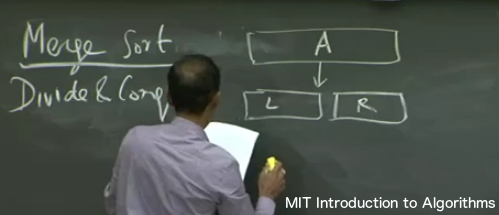
\includegraphics[width=0.55\columnwidth]{img/frontpage-6006.png}
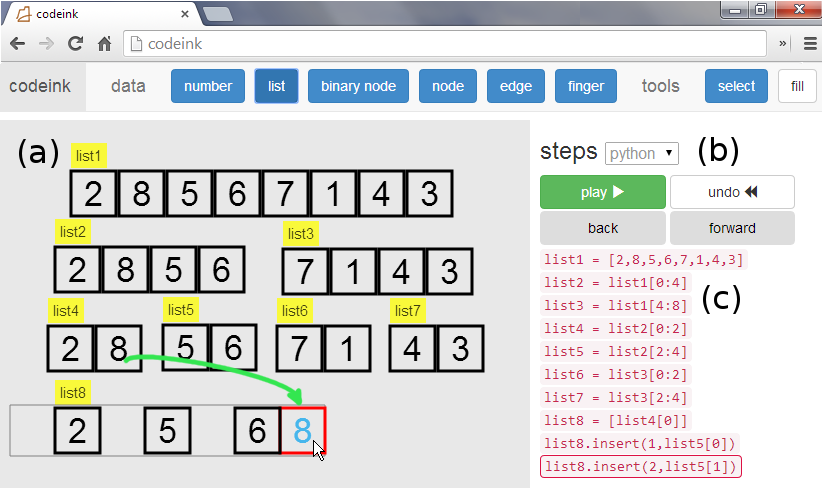
\includegraphics[width=\columnwidth]{img/frontpage-mergesort.png}
\end{center}

\vspace{-0.5em}

\caption{CodeInk is a Web-based tool that implements a direct
manipulation language for tracing algorithms on data structures for the
purpose of CS education. CodeInk allows the user to (a) compose and
manipulate data structures on a graphical canvas, (b) step forward and
backward through the recorded trace, and (c) see each step translated
into a line of Python code or an English explanation.}

%The CodeInk user interface is (a) a canvas for composing and
%manipulating data structures and (c) an interactive list of Python steps
%recorded by the tool, based on the user's interactions. The user can
%step forward and backward through the steps, or replay the entire trace
%using the playback controls (b).}

\label{fig:codeink-intro}
\end{figure}

% Code-driven visualization is for visualization, not explanation or active
% learning Also at the wrong level of abstraction
Code-driven visualization offers an alternative to tracing-by-drawing, where the
user can input an algorithm's code and watch an animation of its execution.
However, watching visualizations is a passive learning process, where tracing
requires the student to play the role of the computer and actively carry out the
algorithm's behavior. Moreover, an algorithm's code is usually at a lower level
of abstraction (language and implementation specific) than the one at which the
algorithm should be explained and learned (language and implementation
agnostic).

We present CodeInk, a CS education tool designed to reduce the tedium and
enhance the experience of tracing algorithms. Using a direct manipulation (DM)
gesture set, users can demonstrate changes to data structures, rather than draw
before and after snapshots. The trace is recorded as an interactive set of
program steps, where each gesture is translated to a line of Python code or
explanatory English. The steps provide several benefits: feedback on user
interactions, navigation through the trace, and a persistent, structured format
that can be easily disseminated and analyzed as a basis for discussion.

For example, an instructor can explain merge sort by dragging an example list
onto the canvas, selecting sublists with a rectangular selection, dragging them
away to create copies, then merging elements by dragging them into a new sorted
list (\fig{fig:codeink-intro}a). Every interaction is interpreted as a step in
Python (\fig{fig:codeink-intro}c). The trace can then be shared with students,
who can navigate through the explanation by clicking on steps
(\fig{fig:codeink-intro}b), and then trace the algorithm for themselves on a new
example. Their own trace can be shared with teachers as a basis for feedback on
not just the final output, but also the process by which the list was sorted.

%We have built CodeInk, a system that enables teachers and students to trace an
%algorithm's behavior by directly manipulating visual objects on a stage. The
%objects represent data structures as they are typically drawn (lists, trees,
%graphs) and can be manipulated using a set of DM gestures to demonstrate
%concrete changes to values and pointer assignments. CodeInk translates all
%interactions into a list of steps, which can be used to navigate through the
%algorithm's trace. In the case where a student is tracing the algorithm's
%behavior, the steps capture their understanding in a structured format, making
%the demonstration analyzable where screencasts, and audio/video recordings are
%not.

This paper makes the following primary contributions:

\begin{enumerate} %\itemsep1pt

\item CodeInk: a CS education tool that enhances the experience of tracing
algorithms on example data structures.
\item A direct manipulation (DM) gesture set for demonstrating changes to list,
tree and graph data structures, where each gesture maps onto a line of Python
code.
\item An evaluation of CodeInk's usability and viability in a controlled study,
where students watched CodeInk-produced traces to learn an algorithm, then used
CodeInk to trace the algorithm for themselves to solidify their
understanding.

\end{enumerate}


\section{Related Work}

Code-driven visualization tools~\cite{Guo2013, Sorva2013} generate
step-by-step animations of code snippet execution. While powerful for
understanding snippets, they are not as good for understanding an
algorithm's high-level behavior, because they work at the wrong level
of abstraction -- i.e., the {\em implementation} of the algorithm in a
particular language. Algorithm visualizations ~\cite{AlgoViz}, address
this problem by operating at an appropriate level of
abstraction, but must be hand-coded for each algorithm.

CodeInk offers an alternative, low-effort method of authoring
visualizations. It also enables students to learn by playing the role of the computer, 
actively tracing algorithm behavior, thereby providing 
active learning, which is known 
to result in better pedagogical outcomes~\cite{Sorva2012Diss}.

% Sorva et al.\ provide a comprehensive survey of 44 such tools
% for languages such as Java, C++, and Python~\cite{Sorva2013}.

%To enable teachers to find and integrate suitable
%visualizations into their curriculula, Shaffer et al.\ created the AlgoViz
%Portal~\cite{AlgoViz}, a website that catalogues and ranks hundreds of existing
%visualizations.

%Shaffer et al.\ surveyed CS instructors and found that while there was high interest in these visualizations, 
% few used them in practice due to the difficulty of finding and integrating
% suitable visualizations into their curriculum~\cite{Shaffer2011}.

Visual programming languages
(e.g.,~\cite{Alice2008},~\cite{Scratch2008}), have a similar spirit,
in enabling writing programs by directly manipulating graphical
elements rather than by typing text. CodeInk differs in intent,
introducing a new visual language that enables users to trace
algorithms by direct manipulation of data structures.

\begin{comment}
Direct manipulation (DM) user interfaces~\cite{Hutchins1985}, starting with
Shneiderman's initial definiton of the term~\cite{Shneiderman1982}, have long
been recognized to promote more satisfactory reactions among users than
command-line or WIMP interfaces. CodeInk's DM gesture set was designed with
these princples in mind: algorithm steps can be described using physical actions
(grabbing and dragging data structures), lowering the degree of indirection
between onscreen objects and the abstract data structures they represent. For
example, list elements can be rearranged by grabbing elements and moving them
into new positions, rather than by writing code or using menus.
\end{comment}

% DM environments for programming by
%demonstration~\cite{Cypher1993} enable users to construct programs by
%demonstrating how the program should behave on specific examples, from which
%% the system refines its understanding of the program. CodeInk's focus is on
% traces of
%algorithms, rather than general programs.


\begin{comment}
Programming by example~\cite{Lieberman2001} enables the user to write programs by
providing example input-output pairs. A related technique, programming by
demonstration~\cite{Cypher1993}, lets the user demonstrate individual steps
using a direct manipulation UI. Tools that embody these techniques often
generalize the user's actions to synthesize programs that operate on new,
unknown inputs~\cite{Yessenov2013, Kandel2011}.
% Common use cases include synthesizing text editing~\cite{Yessenov2013} and
% data cleaning~\cite{Kandel2011} scripts.
CodeInk takes inspiration from these tools and allows the user to explain
algorithms by demonstration, rather than by writing code. CodeInk does not yet
provide generalization capabilities; we plan to add that in future work.
\end{comment}

\section{Design Rationale: Educational use cases}


\begin{figure}
\begin{center}
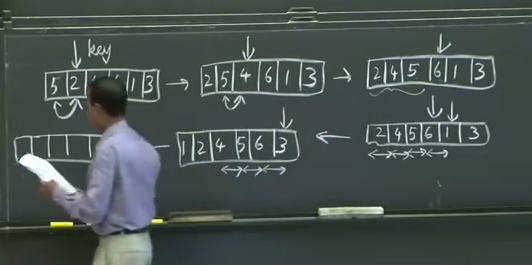
\includegraphics[width=0.7\columnwidth]{img/6006/insertion.png}
\end{center}

\caption{An algorithms instructor traces the operation of insertion sort 
on a concrete example of a list by drawing storyboard snapshots.}

\label{fig:6006-insertion}
\end{figure}


CodeInk's design is inspired 
by  the actions of instructors and by best practices
identified in educational psychology.

One such practice~\cite{Lister2004} found that a student's ability to trace code is a
prerequisite for being adept at problem solving and writing code, suggesting that CS courses should ``first teach systematic tracing as a base
skill, then allow students to build [\ldots]\ upon that''.
% found that students in introductory programming courses could not
% consistently demonstrate an understanding of code by manually tracing
% it. The researchers noted that ``even when our principal aim is to
% teach students to write code, we require students to learn by reading
% code''

We also noted that instructors often start explaining algorithms by
tracing code on concrete examples (\fig{fig:6006-insertion}), rather
than explaining the algorithm in the general case or drawing flow
control.  Instead, they unfold the loops and branches of an
algorithm's pseudocode into a linear sequence of steps.
%%% POSSIBLY PUT BACK IN THE TEXT COMMENTED OUT BELOW?
%%%
% This approach is in line with findings that students need to see multiple
% examples of an algorithm's behavior to build their
% understanding~\cite{Vainio2007}.

In response to both of these observations, CodeInk targets the task of
tracing algorithms behavior on concrete examples, enabling students to
practice tracing examples in an engaging, interactive environment.
The student has the freedom to explore an algorithm's behavior,
perhaps making mistakes along the way.  CodeInk records every action
the student makes, providing a basis for targeted
feedback~\cite{Balzer1989} on both the final answer and the process by
which the student reached their answer.

We further noted that algorithm explanations typically occur at a high
level of abstraction, using pseudocode and diagrams rather than
language-specific code. This abstracts away language-specific details,
a lesson incorporated in CodeInk's goal of enabling the illustration of
algorithm behavior by direct manipulation of data structure diagrams.

Finally, CodeInk uses the visual vocabulary common to programmers, e.g., 
lists drawn as a row of boxes (\fig{fig:6006-insertion}), trees and graphs
drawn as circles connected by arrows. Values are drawn as a number
within or adjacent to each object (Figure 3).\footnote{All examples in our system so far
use numerical data.}

%Also, according to cognitive load theory, novices can learn better by watching
%experts solve problems that would be too difficult for novices to solve on
%% their own~\cite{Linn1992, Sweller1985}. The instructor's worked examples give
%% students
%an opportunity to get the gist of an algorithm, before they attempt to trace it
%on their own. 



\begin{figure}
\begin{center}
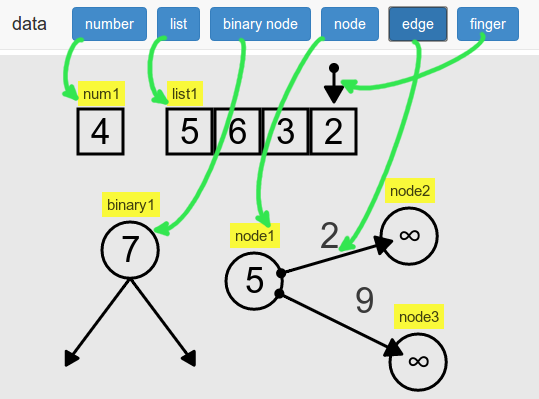
\includegraphics[width=0.8\columnwidth]{img/visual-vocabulary.png}
\end{center}

\caption{CodeInk's visual vocabulary and data palette, located at the
top of the interface. The green arrows are for illustration, and
show how the user can drag data structures (numbers, lists, binary tree
nodes, graph nodes, edges) and visual fingers onto the stage.}
%% strongly suggest getting rid of green arrows; they are confusing and not
%%% needed. Say instead: ``Each of the data structure types at the top can be dragged onto the stage.��
%% also: later in the paper we talk about �the canvas� rather than �stage�.
%% Pick one term and stick to it.
\label{fig:visual_vocab}
\end{figure}


\begin{comment}
Instructors add to this vocabulary using arrows and colors. Arrows are
interchangably used to show transitions between storyboard frames, or to point
to the current focus of the algorithm (\fig{fig:6006-insertion}). The former is
an artifact of the need to draw snapshots when using blackboards, while the
latter is an important visual cue for following the algorithm's progress. Colors
are also used to visualize state; for example, to mark graph nodes as visited,
they are filled with a different color. CodeInk's visual vocabulary includes
\emph{fingers}, which can be attached to any on-screen object, and a \emph{fill}
gesture (explained later) that can be used to color a data structure.
\end{comment}


% Show your work

%Finally, students eventually need to learn to write algorithms in a real
%programming language. CodeInk provides a mapping from visual data
%structure changes to lines of Python code. This serves as a form of
%instructional scaffolding~\cite{Pea2004} to help students acquire
%basic programming skills.

\begin{comment}

CodeInk supports three main educational use cases:

\begin{itemize}\itemsep0pt

\item Instructors can easily create algorithm explanations that can be
used in a live class or disseminated online.

\item Students can step through instructor-created explanations to learn
both the algorithms and basic Python constructs, such as list
manipulation operators.

\item Students can solidify their understanding by tracing an algorithm
on new input data. CodeInk records all user interactions, which enables
instructors to give targeted feedback~\cite{Balzer1989} on the student's
problem-solving process.

\end{itemize}

\end{comment}


%concrete tracing, worked examples, targeted feedback, and instructional
% scaffolding.
%We hypothesize that the ideal user interface for teaching and learning
%algorithms should support exploration by tracing, and enhance the experience by
%(a) affording users the ability to directly manipulate data structures, and
%(b) recording the trace in a structured, persistent format that affords
%dissemination, interaction and discussion.

% CodeInk:
%- Objective: enable teachers and students to explain algorithms by directly
% manipulating data structures.
%- Scope: traces and visual problems
%- Usage model through example
%- Use cases

\section{CodeInk: an algorithm tracing tool}
CodeInk (\fig{fig:codeink-intro}) is a Web-based tool that enables teachers and
students to trace algorithms by direct manipulation. The system consists of
three components: (1) a data palette for constructing examples of data
structures, (2) a DM gesture set for demonstrating changes to the data
structures, and (3) the recorded trace.
% which both enables navigation through the trace and can be disseminated or
% analyzed as a basis for feedback.
Its usage model is the following:

\begin{enumerate}

\item Setup a concrete example of a data structure (number, list, binary tree,
graph) by dragging objects from the data palette onto the canvas and
initializing their values.

\item Directly manipulate the data structure using CodeInk's gesture set to
carry out an algorithm's trace on the example.

\item Every interaction adds a step to the recorded trace, translated into
Python or explanatory English (\fig{fig:codeink-intro}c). Click on any step to
jump to the corresponding point in the trace, or play back the trace using the
controls in \fig{fig:codeink-intro}b.

\item Share the explanation by generating a URL, embedding into a Web page, or
exporting as a video. The trace is machine-readable (lines of Python), meaning
it could be analyzed automatically to provide feedback at scale.

\end{enumerate}

\begin{comment}
\subsection{Data Palette}
The teacher or student begins by setting up an example on which an algorithm
will be traced. This can be done by dragging data structures from the Data
Palette onto the stage (\fig{fig:visual_vocab}). Each data structure can be
initialized by entering a numeric value into a prompt (list elements can be set
by entering a comma-separated list of numbers). CodeInk's current visual
vocabulary supports numeric values, which is sufficient for explaining most
sorting and search algorithms. We discuss extensions of the vocabulary in the
future work section. The \emph{finger} can be used to express the current
traversal point in an algorithm, like a \emph{curr} pointer. In an educational
setting, the finger replaces the instructor pointing to a particular object
during lecture.
\end{comment}

% Included in tool.tex
\subsection{Direct Manipulation (DM) Gesture Set}

\begin{table}[!b]
% % increase table row spacing, adjust to taste
\renewcommand{\arraystretch}{1.75}
% if using array.sty, it might be a good idea to tweak the value of
% \extrarowheight as needed to properly center the text within the cells
% \setlength{\extrarowheight}{10pt}
\centering
% % Some packages, such as MDW tools, offer better commands for making tables %
% than the plain LaTeX2e tabular which is used here.
\begin{tabular}{|p{3.8cm} |p{3.8cm} |}
\hline
\textbf{Algorithm Behavior} & \textbf{DM Gesture} \\
\hline
%Access a value & Grab value and drag elsewhere \\
%\hline
Use or copy an object's value & {\em drag-away}: Grab an object, and drag it
away quickly.
Drop it on the stage to create a new number with the same value.
\\
\hline
Remove an object from its parent (e.g. element from list, node from tree/graph) & {\em dwell-drag-away}: Grab an object, dwell for one second, then
drag it elsewhere.
\\
\hline
Compare two objects' values & {\em drag-into}: Drag one value into another.
\\
\hline
Assign one object's value to another &
{\em drag-into-dwell}: Drag one value into another, and
dwell until the desired interpretation (\texttt{=, +=, -=}) appears. \\
\hline
Insert a value into a list, or a node into a tree/graph
& {\em drag-insert}: Drag the value into a gap in the list, or the node to the
tip of an edge
\\

\hline
Attach an edge to a graph node
& {\em drag-edge}: Drag the edge's start or end handle to the node.
\\

\hline
Mark a list element or tree/graph node (e.g. as sorted or visited) &
{\em fill}: Select the ``Fill" tool, and click on the element. \\
\hline
\end{tabular}

\caption{CodeInk's Direct Manipulation (DM) Gesture Set}
\label{tbl:gesture_table}

\end{table}

CodeInk's DM gesture set (summarized in \tab{tbl:gesture_table}) enables
users to trace algorithms by manipulating numbers, lists, binary trees and
graphs. From our experience of watching online lecture videos of an introductory
algorithms class, we compiled a list of algorithm behaviors that need to be
expressed when tracing commonly taught sorting and search algorithms (left
column of \tab{tbl:gesture_table}).
For each behavior, we then devised a gesture, in keeping with principles of direct
manipulation~\cite{Shneiderman1982, Lee2012}, that would enable the user to
express each behavior using a physical action. For example, numbers can be
copied by grabbing them and dragging away, and they can be inserted into lists
by dragging them into gaps between other elements.

All data structures in CodeInk's visual vocabulary are composed of one
or more objects (list elements or nodes), each with numeric values. For
that reason, the gesture set is both compact (7 gestures in total) and
expressive: dragging one object into another compares their numeric
values, regardless of whether they are numbers, list elements, nodes or
some mixture thereof. Similarly, popping a list element or detaching a
subtree from its parent is accomplished by grabbing and holding it
(\emph{dwelling}) until it can be moved away freely. We explain the
design decision behind dwelling later in this section. We now illustrate
the gesture set through two examples.

\noindent \textbf{Insertion Sort}: An instructor or student typically
traces insertion sort on an example list by redrawing it in successive
configurations (\fig{fig:6006-insertion}). With CodeInk, the algorithm
can be traced as follows:

\noindent 1) Drag an example list onto the stage (main canvas) and enter
numbers to initialize element values. Drag a finger onto the stage to
point to the starting element. The green arrows below indicate user drag
motion and are not part of the CodeInk UI.

\vspace{-0.25em}
\noindent 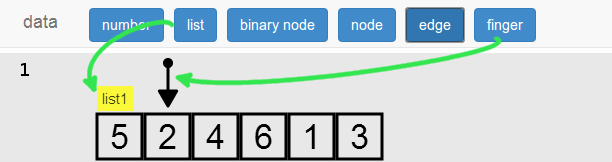
\includegraphics[width=0.7\columnwidth]{img/examples/insertion-1.png}
\vspace{0.5em}

\noindent 2) To prepare to move the ``2" element, grab and hold the element for
at least one second (\emph{dwell}). A blue circle fills up to give the user
feedback on how long they have dwelled.

\vspace{-0.25em}
\noindent 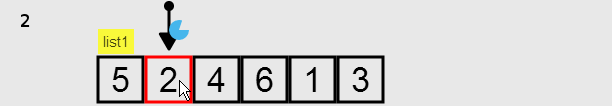
\includegraphics[width=0.7\columnwidth]{img/examples/insertion-2.png}
\vspace{0.4em}

\noindent 3) After one second has elapsed (blue circle filled entirely), the
list expands outward, creating gaps into which the element can be inserted. The
``2" element is now ready to be moved.

\vspace{-0.25em}
\noindent 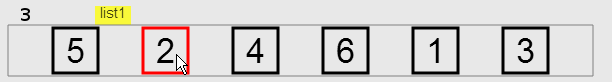
\includegraphics[width=0.7\columnwidth]{img/examples/insertion-3.png}
\vspace{0.5em}

\noindent 4) Drag the ``2" to the left until it hits the ``5" element, which
adds a numeric comparison step (``2 $<$ 5") to the trace.

\vspace{-0.25em}
\noindent 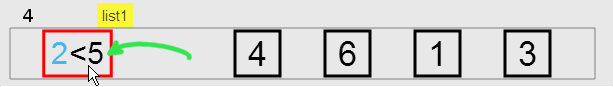
\includegraphics[width=0.7\columnwidth]{img/examples/insertion-4.png}
\vspace{0.5em}

\noindent 5) Keep moving the ``2" to the left of the ``5" element.

\vspace{-0.25em}
\noindent 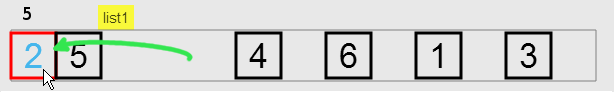
\includegraphics[width=0.7\columnwidth]{img/examples/insertion-5.png}
\vspace{0.5em}

\noindent 6) Once the correct position is found, drop the element
to adds a list insertion step to the trace. The list collapses again in its new, rearranged state, with the
``2" preceeding the ``5''.

\noindent 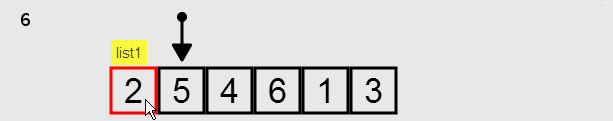
\includegraphics[width=0.7\columnwidth]{img/examples/insertion-6.png}

The user traces the rest of insertion sort by moving the finger down the
list and inserting elements into the sorted sublist until the entire
list is sorted. If any mistakes are made, the user can undo steps to
remove them from the trace.


\noindent \textbf{AVL Insertion}: Drawing an AVL (balanced binary search
tree) insertion can be tedious and error-prone, because rotations
require redrawing the entire tree in a new configuration. CodeInk's
gesture set affords users the ability to rearrange nodes in the tree by
detaching, dragging, and reattaching them. As is the case with lists,
dragging one value into another triggers a numeric comparison (Step 2),
and grabbing and dwelling removes a child from its parent (Step 5).


\noindent \begin{tabular}{m{4.6cm} m{3.4cm}}

1) Create two new binary tree nodes (``4" and ``6") by dragging node
objects onto the stage and typing in their numeric values.

& 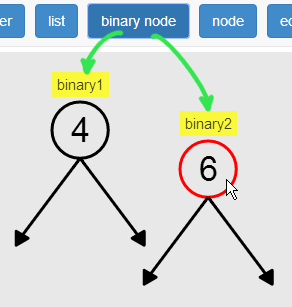
\includegraphics[width=3.4cm]{img/examples/bst-1.png}
\end{tabular}


\noindent \begin{tabular}{m{4.6cm} m{3.4cm}}

2) Drag the ``6'' node into the ``4'' node to compare their values.
CodeInk adds the comparison step (``4 $<$ 6") to the trace.

& 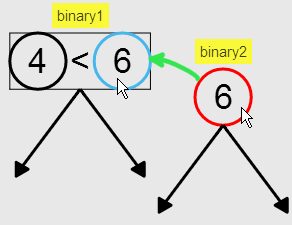
\includegraphics[width=3.4cm]{img/examples/bst-2.png}
\end{tabular}

\noindent \begin{tabular}{m{6.2cm} m{1.8cm}}

3) Since ``6" is greater than ``4", keep dragging the ``6'' along the
right pointer of the ``4" node. This gesture temporarily highlights the pointer
blue and adds a \emph{pointer traversal} step to the trace.

& 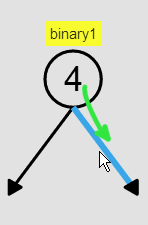
\includegraphics[width=1.8cm]{img/examples/bst-3.png}
\end{tabular}

\noindent \begin{tabular}{m{4.6cm} m{3.4cm}}

4) Keep dragging along the right pointer until reaching its tip. The
``6" node now re-emerges as the right child of ``4." The node is colored blue to
preview the insertion. Release the node to confirm the insertion and
add the step \texttt{binary1.right = binary2} to the trace.

& 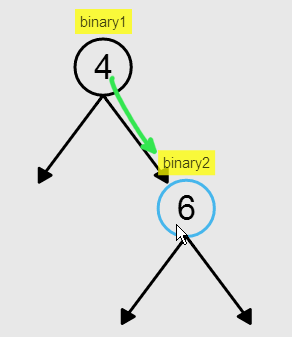
\includegraphics[width=3.4cm]{img/examples/bst-4.png}
\end{tabular}

\noindent \begin{tabular}{m{4.6cm} m{3.4cm}}

5) Next insert a new ``9" node into the tree, which results in an
unbalanced tree. Now demonstrate a rotation by grabbing the ``6" node,
dwelling for one second, and dragging it away to detach the subtree.
When the subtree is dropped on the stage, a new step is added to the
trace: \texttt{binary1.right = None}

& 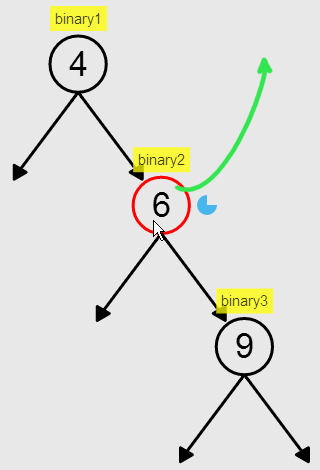
\includegraphics[width=3.4cm]{img/examples/bst-5.png}
\end{tabular}

\noindent \begin{tabular}{m{4.6cm} m{3.4cm}}

6) The ``6 / 9" subtree is now separated from the ``4." Drag the ``4"
node downward ...

& 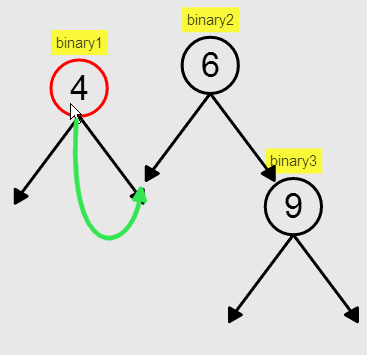
\includegraphics[width=3.4cm]{img/examples/bst-6.png}
\end{tabular}

\noindent \begin{tabular}{m{4.6cm} m{3.4cm}}

7) ... until it reaches the tip of the ``6" node's left pointer. Then
release to insert it there and balance the tree, thereby adding the step
\texttt{binary2.left = binary1} to the trace.

& 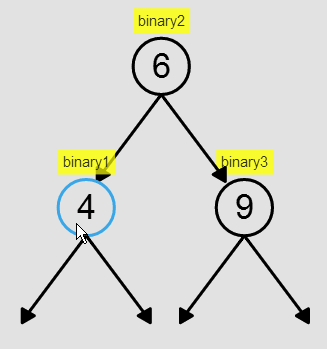
\includegraphics[width=3.4cm]{img/examples/bst-7.png}
\end{tabular}

\begin{comment}
\noindent \textbf{Graph algorithms}: Our gesture set also covers graph
traversal, such as search or finding shortest paths (see
\fig{fig:example-dijkstra}). It supports creating and attaching graph
nodes and edges, updating node and edge values, and marking nodes as
visited. Here is how to trace Dijkstra's algorithm using CodeInk:

\noindent \begin{tabular}{m{4.2cm} m{3.8cm}}
1) Create an example graph by dragging and dropping node and edge
objects onto the stage, typing in the numeric node costs and edge weights.
Edges can be connected to nodes by clicking and dragging their start and end
handles.
& 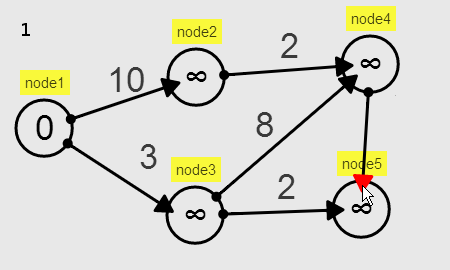
\includegraphics[width=3.8cm]{img/examples/dijkstra-1.png}
\end{tabular}

\noindent \begin{tabular}{m{4.2cm} m{3.8cm}}
2) Start with \texttt{node1}. To calculate the
cost of reaching its neighbor \texttt{node2},
first drag \texttt{node1} (source node) and drop it onto the stage, which
creates a new number (\texttt{num1}) equal to the node's cost (\texttt{0}).
& 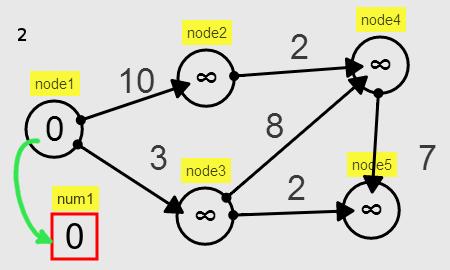
\includegraphics[width=3.8cm]{img/examples/dijkstra-2.png}
\end{tabular}

\noindent \begin{tabular}{m{4.2cm} m{3.8cm}}
3) Now drag the weight of the connecting edge into the current cost
(\texttt{num1}), which triggers a comparison by default. However, a
comparison is not the correct operation; the two values
must be added.
& 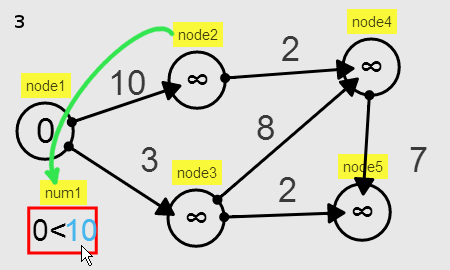
\includegraphics[width=3.8cm]{img/examples/dijkstra-3.png}
\end{tabular}

\noindent \begin{tabular}{m{4.2cm} m{3.8cm}}
4) Dwelling after the drag-into gesture causes CodeInk to cycle through alternative
interpretations. When an addition assignment
operation (\texttt{+=}) appears, release to end the gesture. The cost
updates to the value of \texttt{10} (\texttt{num1 += edge1.weight}).
& 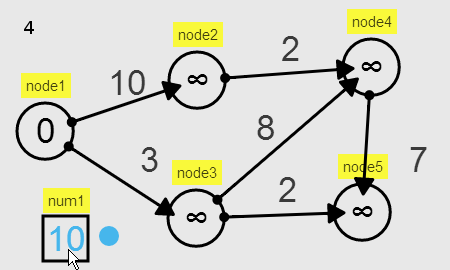
\includegraphics[width=3.8cm]{img/examples/dijkstra-4.png}
\end{tabular}

\noindent \begin{tabular}{m{4.2cm} m{3.8cm}}
5) Now drag \texttt{num1} into \texttt{node2}
to trigger a comparison, checking if the new cost is less than
the existing cost of reaching that node.
& 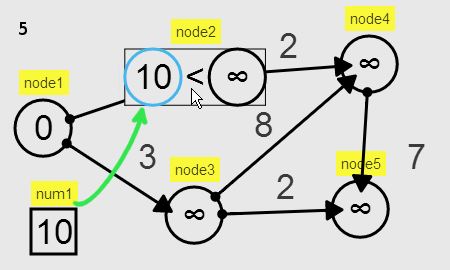
\includegraphics[width=3.8cm]{img/examples/dijkstra-5.png}
\end{tabular}

\noindent \begin{tabular}{m{4.2cm} m{3.8cm}}
6) Since \texttt{10 $<$ $\infty$}, dwell to cycle to the assignment
expression (\texttt{node2.value = num1}). Releasing ends the gesture, and updates the cost
of \texttt{node2} to 10.
& 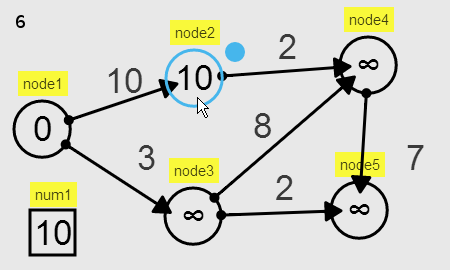
\includegraphics[width=3.8cm]{img/examples/dijkstra-6.png}
\end{tabular}

\noindent \begin{tabular}{m{4.2cm} m{3.8cm}}
7) Repeat on all nodes and mark each one as visited by
selecting ``Fill" and clicking on that node.
& 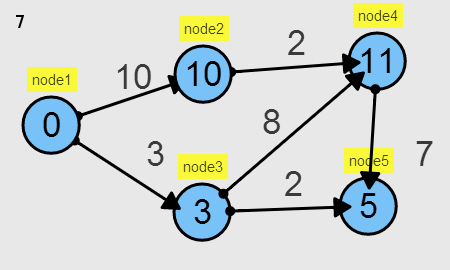
\includegraphics[width=3.8cm]{img/examples/dijkstra-7.png}
\end{tabular}

%Because the drag-into gesture has multiple interpretations
%(comparison, assignment, addition assignment), the user can dwell
%to cycle through all interpretations (see \sec{sec:overloaded-gestures}).
\end{comment}

\subsection{Chaining and traversal patterns}
In CodeInk, the user can chain multiple gestures while dragging an object to
describe a traversal pattern. For example, during insertion sort, the user can
drag an element along the list, performing comparisons without releasing it
until the correct location is found. Similarly, during an AVL insertion, a
candidate node is dragged through the tree to make comparisons and follow
pointers to find the insertion point.

One subtle interaction issue is deciding which behaviors in a chain of
gestures to commit (add) to the trace. For example, the user should be
allowed to click and drag an element into a list, then undo the behavior
by dragging it back out before releasing the mouse button. The insertion
step should be committed only if the new value is released into the
list, but comparisons should be committed as the user is dragging the
element as part of a traversal pattern. We therefore distinguish between
\emph{mutation} and \emph{observation} behaviors as those that affect
the underlying data and those that only visualize decision making in the
algorithm, respectively. In a chain of gestures, observation behaviors
(e.g., comparisons) are continuously committed to the trace, while
mutation behaviors (e.g., insertions) are committed only at the end of a
gesture.

\subsection{Resolving overloaded gestures}
\label{sec:overloaded-gestures}

% When designing a gesture vocabulary, the gesture that seems most
% natural for a task can often be interpreted in multiple ways.
\tab{tbl:gesture_table} shows two overloaded gestures: drag-into and
drag-away. Drag-into is ambiguous because dragging one object into
another could be interpreted as a comparison (\texttt{x$<$y}) or an
assignment (\texttt{x=y}).
% or an augmented assignment such as \texttt{x+=y} or \texttt{x-=y}.
Performing the drag-away gesture on a child object is ambiguous because
it is not obvious whether the parent object should be altered. For
example, when dragging an element away from a list, should a copy of the
element be made, or should the element be popped from the parent list?
% For trees and graphs, should a copy of the dragged node be made, or
% should that node and its descendants be detached from the parent?
%
Our solution defaults to safe observation behaviors and previews other
possible mutation behaviors if the user dwells -- grabs and holds the
object -- for more than one second.
% This means defaulting to a comparison for the drag-into gesture, and
% making a copy of the dragged value for the drag-away gesture.
This design also aligns well with chained traversal patterns, since
comparisons can occur in quick succession while dragging.



\subsection{Recorded Trace}

%Each gesture is translated to a line of Python or
%explanatory English, effectively recording the trace as a set of program steps.
% The steps are interactive, enabling the user to navigate through the trace by
% single-stepping
%or clicking to jump between steps. The recorded trace can also be shared
% between teachers and students, enabling dissemnation, discussion and feedback.

\subsection{Scope: concrete traces and visual problems}
% unfolding of the loops and branches in an algorithm's pseudocode
Second, this work focuses on supporting traces on lists, binary trees, and
graphs, because their canonical algorithms -- sorting, rotation, search and
shortest paths -- are widely taught in introductory CS and algorithms classes.
These data structures and their associated algorithms are also inherently
visual: The natural way to teach and think through them is by drawing diagrams.
Thus, we envision direct manipulation for tracing to be most useful for these
types of problems.
% Also, they represent around \todo{50\%} of the algorithms covered in
% CLRS~\cite{Cormen2001}, one of the most popular algorithms textbooks.
In \sec{sec:design-and-future-work}, we discuss how our language can be extended
to support demonstrations of an algorithm's general behavior across more kinds
of data structures.

% Included in tool.tex
\subsection{Direct Manipulation (DM) Gesture Set}

\begin{table}[!b]
% % increase table row spacing, adjust to taste
\renewcommand{\arraystretch}{1.75}
% if using array.sty, it might be a good idea to tweak the value of
% \extrarowheight as needed to properly center the text within the cells
% \setlength{\extrarowheight}{10pt}
\centering
% % Some packages, such as MDW tools, offer better commands for making tables %
% than the plain LaTeX2e tabular which is used here.
\begin{tabular}{|p{3.8cm} |p{3.8cm} |}
\hline
\textbf{Algorithm Behavior} & \textbf{DM Gesture} \\
\hline
%Access a value & Grab value and drag elsewhere \\
%\hline
Use or copy an object's value & {\em drag-away}: Grab an object, and drag it
away quickly.
Drop it on the stage to create a new number with the same value.
\\
\hline
Remove an object from its parent (e.g. element from list, node from tree/graph) & {\em dwell-drag-away}: Grab an object, dwell for one second, then
drag it elsewhere.
\\
\hline
Compare two objects' values & {\em drag-into}: Drag one value into another.
\\
\hline
Assign one object's value to another &
{\em drag-into-dwell}: Drag one value into another, and
dwell until the desired interpretation (\texttt{=, +=, -=}) appears. \\
\hline
Insert a value into a list, or a node into a tree/graph
& {\em drag-insert}: Drag the value into a gap in the list, or the node to the
tip of an edge
\\

\hline
Attach an edge to a graph node
& {\em drag-edge}: Drag the edge's start or end handle to the node.
\\

\hline
Mark a list element or tree/graph node (e.g. as sorted or visited) &
{\em fill}: Select the ``Fill" tool, and click on the element. \\
\hline
\end{tabular}

\caption{CodeInk's Direct Manipulation (DM) Gesture Set}
\label{tbl:gesture_table}

\end{table}

CodeInk's DM gesture set (summarized in \tab{tbl:gesture_table}) enables
users to trace algorithms by manipulating numbers, lists, binary trees and
graphs. From our experience of watching online lecture videos of an introductory
algorithms class, we compiled a list of algorithm behaviors that need to be
expressed when tracing commonly taught sorting and search algorithms (left
column of \tab{tbl:gesture_table}).
For each behavior, we then devised a gesture, in keeping with principles of direct
manipulation~\cite{Shneiderman1982, Lee2012}, that would enable the user to
express each behavior using a physical action. For example, numbers can be
copied by grabbing them and dragging away, and they can be inserted into lists
by dragging them into gaps between other elements.

All data structures in CodeInk's visual vocabulary are composed of one
or more objects (list elements or nodes), each with numeric values. For
that reason, the gesture set is both compact (7 gestures in total) and
expressive: dragging one object into another compares their numeric
values, regardless of whether they are numbers, list elements, nodes or
some mixture thereof. Similarly, popping a list element or detaching a
subtree from its parent is accomplished by grabbing and holding it
(\emph{dwelling}) until it can be moved away freely. We explain the
design decision behind dwelling later in this section. We now illustrate
the gesture set through two examples.

\noindent \textbf{Insertion Sort}: An instructor or student typically
traces insertion sort on an example list by redrawing it in successive
configurations (\fig{fig:6006-insertion}). With CodeInk, the algorithm
can be traced as follows:

\noindent 1) Drag an example list onto the stage (main canvas) and enter
numbers to initialize element values. Drag a finger onto the stage to
point to the starting element. The green arrows below indicate user drag
motion and are not part of the CodeInk UI.

\vspace{-0.25em}
\noindent 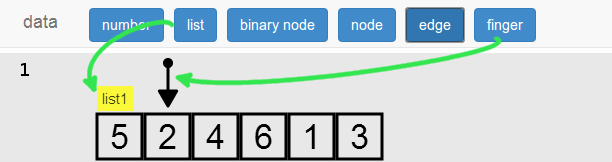
\includegraphics[width=0.7\columnwidth]{img/examples/insertion-1.png}
\vspace{0.5em}

\noindent 2) To prepare to move the ``2" element, grab and hold the element for
at least one second (\emph{dwell}). A blue circle fills up to give the user
feedback on how long they have dwelled.

\vspace{-0.25em}
\noindent 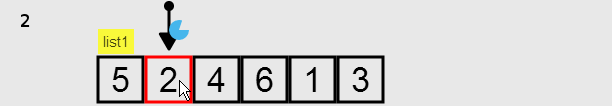
\includegraphics[width=0.7\columnwidth]{img/examples/insertion-2.png}
\vspace{0.4em}

\noindent 3) After one second has elapsed (blue circle filled entirely), the
list expands outward, creating gaps into which the element can be inserted. The
``2" element is now ready to be moved.

\vspace{-0.25em}
\noindent 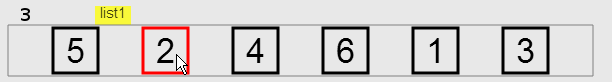
\includegraphics[width=0.7\columnwidth]{img/examples/insertion-3.png}
\vspace{0.5em}

\noindent 4) Drag the ``2" to the left until it hits the ``5" element, which
adds a numeric comparison step (``2 $<$ 5") to the trace.

\vspace{-0.25em}
\noindent 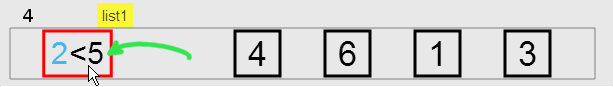
\includegraphics[width=0.7\columnwidth]{img/examples/insertion-4.png}
\vspace{0.5em}

\noindent 5) Keep moving the ``2" to the left of the ``5" element.

\vspace{-0.25em}
\noindent 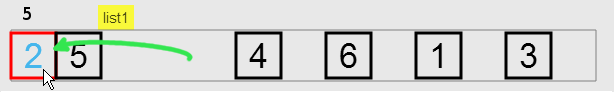
\includegraphics[width=0.7\columnwidth]{img/examples/insertion-5.png}
\vspace{0.5em}

\noindent 6) Once the correct position is found, drop the element
to adds a list insertion step to the trace. The list collapses again in its new, rearranged state, with the
``2" preceeding the ``5''.

\noindent 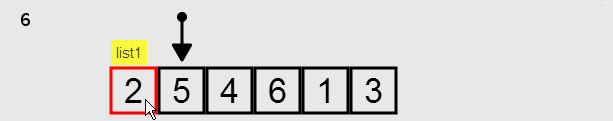
\includegraphics[width=0.7\columnwidth]{img/examples/insertion-6.png}

The user traces the rest of insertion sort by moving the finger down the
list and inserting elements into the sorted sublist until the entire
list is sorted. If any mistakes are made, the user can undo steps to
remove them from the trace.


\noindent \textbf{AVL Insertion}: Drawing an AVL (balanced binary search
tree) insertion can be tedious and error-prone, because rotations
require redrawing the entire tree in a new configuration. CodeInk's
gesture set affords users the ability to rearrange nodes in the tree by
detaching, dragging, and reattaching them. As is the case with lists,
dragging one value into another triggers a numeric comparison (Step 2),
and grabbing and dwelling removes a child from its parent (Step 5).


\noindent \begin{tabular}{m{4.6cm} m{3.4cm}}

1) Create two new binary tree nodes (``4" and ``6") by dragging node
objects onto the stage and typing in their numeric values.

& 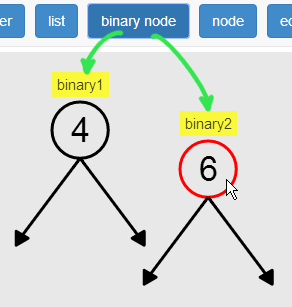
\includegraphics[width=3.4cm]{img/examples/bst-1.png}
\end{tabular}


\noindent \begin{tabular}{m{4.6cm} m{3.4cm}}

2) Drag the ``6'' node into the ``4'' node to compare their values.
CodeInk adds the comparison step (``4 $<$ 6") to the trace.

& 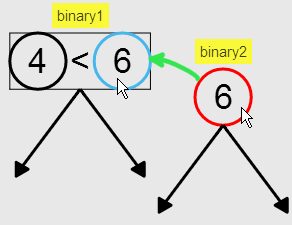
\includegraphics[width=3.4cm]{img/examples/bst-2.png}
\end{tabular}

\noindent \begin{tabular}{m{6.2cm} m{1.8cm}}

3) Since ``6" is greater than ``4", keep dragging the ``6'' along the
right pointer of the ``4" node. This gesture temporarily highlights the pointer
blue and adds a \emph{pointer traversal} step to the trace.

& 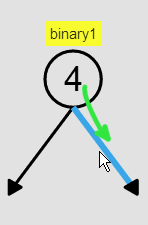
\includegraphics[width=1.8cm]{img/examples/bst-3.png}
\end{tabular}

\noindent \begin{tabular}{m{4.6cm} m{3.4cm}}

4) Keep dragging along the right pointer until reaching its tip. The
``6" node now re-emerges as the right child of ``4." The node is colored blue to
preview the insertion. Release the node to confirm the insertion and
add the step \texttt{binary1.right = binary2} to the trace.

& 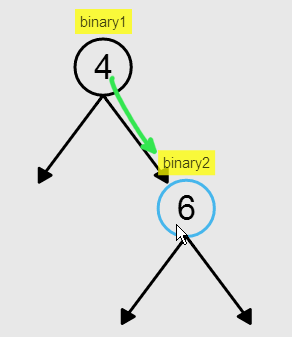
\includegraphics[width=3.4cm]{img/examples/bst-4.png}
\end{tabular}

\noindent \begin{tabular}{m{4.6cm} m{3.4cm}}

5) Next insert a new ``9" node into the tree, which results in an
unbalanced tree. Now demonstrate a rotation by grabbing the ``6" node,
dwelling for one second, and dragging it away to detach the subtree.
When the subtree is dropped on the stage, a new step is added to the
trace: \texttt{binary1.right = None}

& 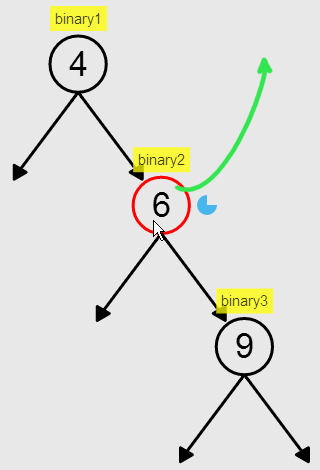
\includegraphics[width=3.4cm]{img/examples/bst-5.png}
\end{tabular}

\noindent \begin{tabular}{m{4.6cm} m{3.4cm}}

6) The ``6 / 9" subtree is now separated from the ``4." Drag the ``4"
node downward ...

& 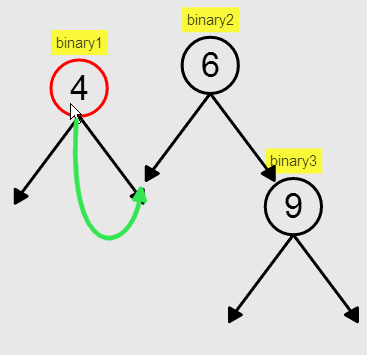
\includegraphics[width=3.4cm]{img/examples/bst-6.png}
\end{tabular}

\noindent \begin{tabular}{m{4.6cm} m{3.4cm}}

7) ... until it reaches the tip of the ``6" node's left pointer. Then
release to insert it there and balance the tree, thereby adding the step
\texttt{binary2.left = binary1} to the trace.

& 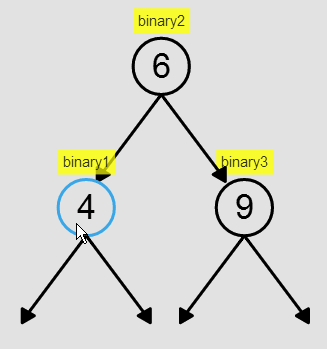
\includegraphics[width=3.4cm]{img/examples/bst-7.png}
\end{tabular}

\begin{comment}
\noindent \textbf{Graph algorithms}: Our gesture set also covers graph
traversal, such as search or finding shortest paths (see
\fig{fig:example-dijkstra}). It supports creating and attaching graph
nodes and edges, updating node and edge values, and marking nodes as
visited. Here is how to trace Dijkstra's algorithm using CodeInk:

\noindent \begin{tabular}{m{4.2cm} m{3.8cm}}
1) Create an example graph by dragging and dropping node and edge
objects onto the stage, typing in the numeric node costs and edge weights.
Edges can be connected to nodes by clicking and dragging their start and end
handles.
& 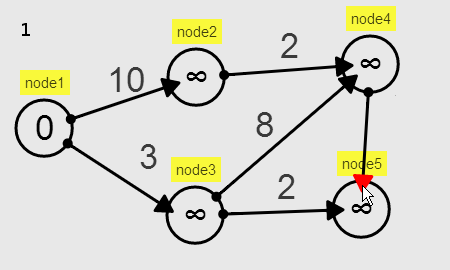
\includegraphics[width=3.8cm]{img/examples/dijkstra-1.png}
\end{tabular}

\noindent \begin{tabular}{m{4.2cm} m{3.8cm}}
2) Start with \texttt{node1}. To calculate the
cost of reaching its neighbor \texttt{node2},
first drag \texttt{node1} (source node) and drop it onto the stage, which
creates a new number (\texttt{num1}) equal to the node's cost (\texttt{0}).
& 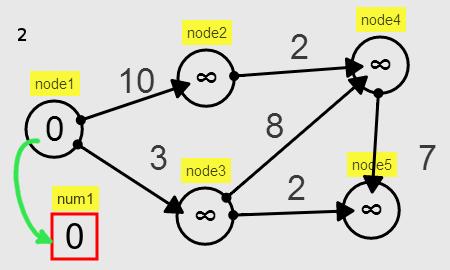
\includegraphics[width=3.8cm]{img/examples/dijkstra-2.png}
\end{tabular}

\noindent \begin{tabular}{m{4.2cm} m{3.8cm}}
3) Now drag the weight of the connecting edge into the current cost
(\texttt{num1}), which triggers a comparison by default. However, a
comparison is not the correct operation; the two values
must be added.
& 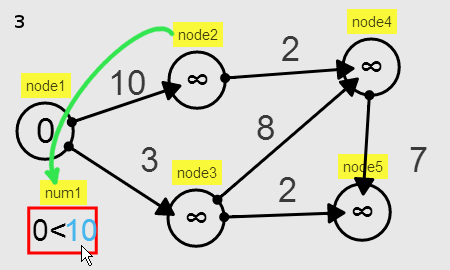
\includegraphics[width=3.8cm]{img/examples/dijkstra-3.png}
\end{tabular}

\noindent \begin{tabular}{m{4.2cm} m{3.8cm}}
4) Dwelling after the drag-into gesture causes CodeInk to cycle through alternative
interpretations. When an addition assignment
operation (\texttt{+=}) appears, release to end the gesture. The cost
updates to the value of \texttt{10} (\texttt{num1 += edge1.weight}).
& 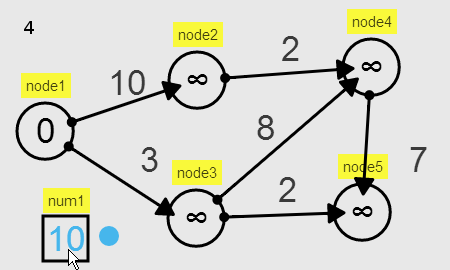
\includegraphics[width=3.8cm]{img/examples/dijkstra-4.png}
\end{tabular}

\noindent \begin{tabular}{m{4.2cm} m{3.8cm}}
5) Now drag \texttt{num1} into \texttt{node2}
to trigger a comparison, checking if the new cost is less than
the existing cost of reaching that node.
& 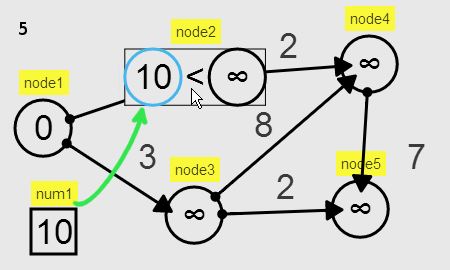
\includegraphics[width=3.8cm]{img/examples/dijkstra-5.png}
\end{tabular}

\noindent \begin{tabular}{m{4.2cm} m{3.8cm}}
6) Since \texttt{10 $<$ $\infty$}, dwell to cycle to the assignment
expression (\texttt{node2.value = num1}). Releasing ends the gesture, and updates the cost
of \texttt{node2} to 10.
& 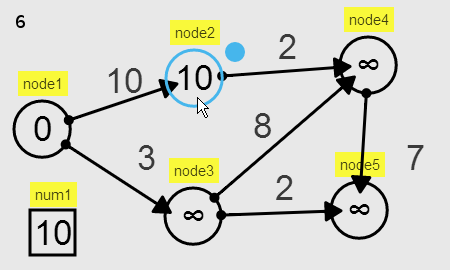
\includegraphics[width=3.8cm]{img/examples/dijkstra-6.png}
\end{tabular}

\noindent \begin{tabular}{m{4.2cm} m{3.8cm}}
7) Repeat on all nodes and mark each one as visited by
selecting ``Fill" and clicking on that node.
& 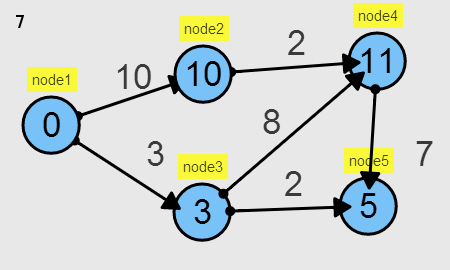
\includegraphics[width=3.8cm]{img/examples/dijkstra-7.png}
\end{tabular}

%Because the drag-into gesture has multiple interpretations
%(comparison, assignment, addition assignment), the user can dwell
%to cycle through all interpretations (see \sec{sec:overloaded-gestures}).
\end{comment}

\subsection{Chaining and traversal patterns}
In CodeInk, the user can chain multiple gestures while dragging an object to
describe a traversal pattern. For example, during insertion sort, the user can
drag an element along the list, performing comparisons without releasing it
until the correct location is found. Similarly, during an AVL insertion, a
candidate node is dragged through the tree to make comparisons and follow
pointers to find the insertion point.

One subtle interaction issue is deciding which behaviors in a chain of
gestures to commit (add) to the trace. For example, the user should be
allowed to click and drag an element into a list, then undo the behavior
by dragging it back out before releasing the mouse button. The insertion
step should be committed only if the new value is released into the
list, but comparisons should be committed as the user is dragging the
element as part of a traversal pattern. We therefore distinguish between
\emph{mutation} and \emph{observation} behaviors as those that affect
the underlying data and those that only visualize decision making in the
algorithm, respectively. In a chain of gestures, observation behaviors
(e.g., comparisons) are continuously committed to the trace, while
mutation behaviors (e.g., insertions) are committed only at the end of a
gesture.

\subsection{Resolving overloaded gestures}
\label{sec:overloaded-gestures}

% When designing a gesture vocabulary, the gesture that seems most
% natural for a task can often be interpreted in multiple ways.
\tab{tbl:gesture_table} shows two overloaded gestures: drag-into and
drag-away. Drag-into is ambiguous because dragging one object into
another could be interpreted as a comparison (\texttt{x$<$y}) or an
assignment (\texttt{x=y}).
% or an augmented assignment such as \texttt{x+=y} or \texttt{x-=y}.
Performing the drag-away gesture on a child object is ambiguous because
it is not obvious whether the parent object should be altered. For
example, when dragging an element away from a list, should a copy of the
element be made, or should the element be popped from the parent list?
% For trees and graphs, should a copy of the dragged node be made, or
% should that node and its descendants be detached from the parent?
%
Our solution defaults to safe observation behaviors and previews other
possible mutation behaviors if the user dwells -- grabs and holds the
object -- for more than one second.
% This means defaulting to a comparison for the drag-into gesture, and
% making a copy of the dragged value for the drag-away gesture.
This design also aligns well with chained traversal patterns, since
comparisons can occur in quick succession while dragging.


\section{Initial Evaluation}

% Testing a novel learning interaction, where students watch a
% CodeInk-produced trace of an algorithm, then trace the algorithm for
% themselves on new examples in the same environment
A formative study of our earlier DM gesture set~\cite{Scott2014} showed
that instructors found CodeInk easier to use and more helpful than a
computer drawing application for explaining list sorting algorithms. In
this initial study, we evaluated two hypotheses about CodeInk's
viability for CS students:

\noindent \textbf{H1}: Students learn as effectively from a
CodeInk-produced explanation as they do from a standard lecture video.

\noindent \textbf{H2}: Students are able to correctly trace the learned
algorithm on a new example data structure.

\noindent \textbf{Subjects}: We recruited nine students from the
introductory programming class at our university. Before the study
began, we asked subjects to rate their initial understanding of lists,
insertion sort, and merge sort on a 7-point Likert scale, based on how
well they could explain the concept to another person. The mean age was
20 ($\sigma$=3.12), with 2 males and 7 females. The mean self-reported
understanding for lists was 2.89 ($\sigma$=2.37). 8 out of 9 students
had never seen insertion or merge sort before (mean understanding =
1.22, $\sigma$=0.67).

\noindent \textbf{Tasks and Procedures}: Each subject began the
30-minute study by watching a training video and getting familiar with
CodeInk's UI and DM gesture set. Students then performed the main task
twice, once for insertion sort and once for merge sort. First, they
learned about the algorithm by watching a video ({\em learning phase})
and then explained its trace on a different list back to the
experimenter ({\em explanation phase}).

In the learning phase, the video was either a screencast of a
CodeInk-produced trace or an excerpt from a classroom lecture
video, where an instructor traces the sorting algorithm on an example
list on the blackboard (\fig{fig:6006-insertion}). The CodeInk-produced
trace covered the exact same examples as the lecture videos. After this
phase, the student was asked to rate their new understanding of the
algorithm on a 7-point Likert scale. In the explanation phase, the
student used CodeInk to trace the algorithm on a new list.

% After the main task, subjects filled out an exit questionnaire, rating the
% helpfulness of three key CodeInk features: the direct manipulation language,
% visualizations of comparisons, and having the trace recorded as a list of
% Python steps.

\noindent \textbf{Results}: Our study supported \textbf{H1}. Recall that
8 out of 9 students reported they had never before seen insertion sort
or merge sort. After the learning phase, students reported that they
learned equally well from a CodeInk-produced traces (mean understanding
= 6.00) as they did from a standard lecture video (mean = 5.56). The
difference was not statistically significant (p=0.196 using a
Mann-Whitney U test). \textbf{H2} was also supported, because all
students who watched the CodeInk-produced trace could then use CodeInk
to trace both insertion sort and merge sort correctly on the new list.

%That is, both the process and final output demonstrated in their traces
%were correct.

%In other words, we found no evidence that CodeInk is any more or less effective
%than a standard online lecture video for teaching these particular algorithms.

This initial study suggests the potential for a new kind of learning
workflow, where CodeInk explanations can be embedded in online course
content. Students can learn about algorithms and practice tracing their
behavior in the same environment. Their traces could then be shared and
analyzed by teaching staff, manually or automatically, as a basis for
targeted feedback~\cite{Balzer1989} on the student's understanding.


\section{Limitations and Future Work}
\label{sec:design-and-future-work}
CodeInk's DM language supports traces of sorting and search algorithms across
lists, binary trees, and graphs. These algorithms comprise roughly one third of
the algorithms in CLRS~\cite{Cormen2001}: comparison sorts, operations on binary
search and red-black trees, breadth-first and depth-first graph traversal and
some shortest path algorithms. To provide completeness for the educational
domain, we plan to extend CodeInk's vocabulary to support additional data
structures (strings, linked lists, hash tables, and 2D arrays), as well as
compound data structures (lists of nodes, for example). This would enable traces
of a broader class of algorithms (dynamic programming, matrix operations), and
more complex traces (maintaining a queue of nodes in a breadth-first traversal).

Importantly, there is a distinction between tracing algorithms and describing
general programs. CodeInk's current focus is on the former, which is well-suited
for teaching algorithms via concrete traces. However, it is essential for
students to build an understanding of control abstraction: iteration sequences,
branching conditions, and recursion. We plan to extend CodeInk's vocabulary to
include gestures for specifying flow control. For example, we are prototyping
gestures for describing iteration by tapping objects and controlling the loop's
execution by dragging a slider between those objects. Our vision is to bring
CodeInk beyond descriptions of algorithm traces, to bridge the gap from concrete
examples to abstract program behavior.


\section{Conclusion}

This paper presents the design of \emph{CodeInk}, a Web-based system for
tracing algorithms by direct manipulation (DM) of data structures. Its
DM gesture set enables users to transform lists, trees, and graphs
rather than having to tediously draw storyboards of an algorithm's
behavior on blackboards or paper. The user-described trace is recorded
as interactive program steps, in Python or explanatory English, which
enable navigation through the trace and can be shared and used as a
basis for targeted feedback. In an initial study that evaluated
CodeInk's viability as a tool in CS education, we found that students
were able to learn as effectively from a CodeInk-produced explanation as
from standard lecture videos, and that they could use CodeInk to trace
the learned algorithm on new example data structures.

%We plan to extend the coverage of CodeInk's vocabulary to more data
%structures and algorithms. We are also prototyping gestures for flow
%control as a step toward an environment for describing general programs,
%not just concrete traces, by direct manipulation.


% use section* for acknowledgement

%\section*{Acknowledgments} The authors would like to thank Rob Miller,
%Tom Lieber, Juho Kim, Carrie Cai, Elena Glassman, the UID group at MIT
%CSAIL and all our study participants for their feedback. This work was
%funded in part by Quanta Computer and NSF. \todo{put the exact grant
%number from the COUHES form}

% references section

% Balancing columns in a ref list is a bit of a pain because you
% either use a hack like flushend or balance, or manually insert
% a column break.  http://www.tex.ac.uk/cgi-bin/texfaq2html?label=balance
% multicols doesn't work because we're already in two-column mode,
% and flushend isn't awesome, so I choose balance.  See this
% for more info: http://cs.brown.edu/system/software/latex/doc/balance.pdf
%
% Note that in a perfect world balance wants to be in the first
% column of the last page.
%
% If balance doesn't work for you, you can remove that and
% hard-code a column break into the bbl file right before you
% submit:
%
% http://stackoverflow.com/questions/2149854/how-to-manually-equalize-columns-
% in-an-ieee-paper-if-using-bibtex
%
% Or, just remove \balance and give up on balancing the last page.
%
\balance

% REFERENCES FORMAT
% References must be the same font size as other body text.
\bibliographystyle{acm-sigchi}
\bibliography{codeinkUIST}


% that's all folks
\end{document}
